\documentclass{beamer}
\mode<presentation>
\usepackage{amssymb}
\usepackage{adjustbox}
\usepackage{booktabs}
\usepackage{subcaption}
\usepackage{multicol}
\usepackage{listings}
\usepackage{graphicx}
\usetheme{AnnArbor}
\usecolortheme{dolphin}
\setbeamertemplate{navigation symbols}
{
  \leavevmode%
  \hbox{%
  \begin{beamercolorbox}[wd=\paperwidth,ht=2.25ex,dp=1ex,right]{author in head/foot}%
    \insertframenumber{} / \inserttotalframenumber\hspace*{2ex} 
  \end{beamercolorbox}}%
  \vskip0pt%
}
\setbeamertemplate{navigation symbols}{}
\lstset{
%language=C,
frame=single, 
breaklines=true,
columns=fullflexible
}
\numberwithin{equation}{section}
\title{ ANSWER TO GATE EC2012 20TH QUESTION}
\author{Srinitha Beerelly}
\date{5 JAN , 2021} 

\begin{document}
\begin{frame}
\titlepage
\begin{corner}
\includegraphics[width=50,height=50]{gate.jpeg}
\end{corner}
\end{frame}

\section*{Outline}
\begin{frame}
\tableofcontents
\begin{corner}
\includegraphics[width=50,height=50]{gate.jpeg}
\end{corner}
\end{frame}
\section{Problem Statement}
\begin{frame}
\frametitle{Problem Statement}
%
Consider the given circuit
\break

\begin{center}
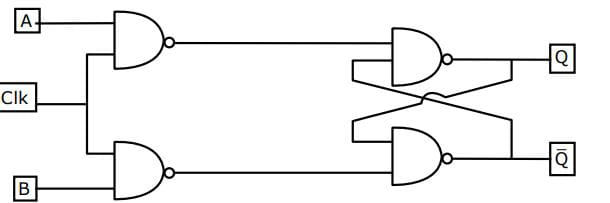
\includegraphics[width=150,height=50]{CIRCUIT.jpeg}
\end{center}


in this circuits, the race around \\
(A) does not occur\\
(B) occurs when CLK=0\\
(C) occurs when CLK=1 and A=B=1\\
(D) occurs when CLK=1 and A=B=0\\
\begin{corner}
\includegraphics[width=50,height=50]{gate.jpeg}
\end{corner}

\end{frame}

\section{solution}
\subsection{circuit diagram}
\begin{frame}
\begin{center}
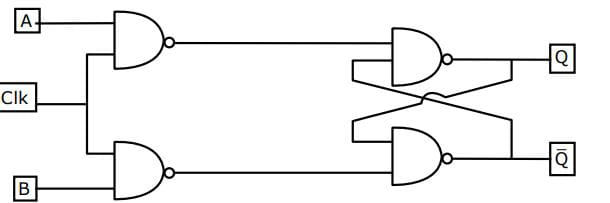
\includegraphics[width=150,height=50]{CIRCUIT.jpeg}
\end{center}




\begin{corner}
\includegraphics[width=50,height=50]{gate.jpeg}
\end{corner}
\end{frame}
\subsection{Explanation}
\begin{frame}
\frametitle{Explanation}

Q_n_e_x_t = \overline{\overline{A.CLK}.{\overline{Q}}}\\
=A.CLK + Q\\
\overline{Q}_n_e_x_t = B.CLK + \overline{Q}\\
If  CLK = 1 and  A = B =1\\
then  Q_n_e_x_t = 1\\
\overline{Q}_n_e_x_t =1\\
then  no  race  around\\
If CLK = 1 and A = B =0\\
then  Q_n_e_x_t = Q\\
\overline{Q}_n_e_x_t = \overline{Q}\\
then no race around\\
Thus race around does not occur in the circuit

\begin{corner}
\includegraphics[width=50,height=50]{gate.jpeg}
\end{corner}
\end{frame}

\subsection{Answer}
\begin{frame}
\frametitle{Answer}

the answer to the given question is (A)

\\
\begin{center}
\underline{To Be Noted} : Race around is applicable only for J-K flip flop when CLK = 1 and A=B=1. But the given circuit is S-R flip flop so no race around occurs.
\end{center}                         

\begin{corner}
\includegraphics[width=50,height=50]{gate.jpeg}
\end{corner}
\end{frame}



\subsection{STATE TRANSITION TABLE}
\begin{frame}
\frametitle{STATE TRANSITION TABLE}

\begin{center}
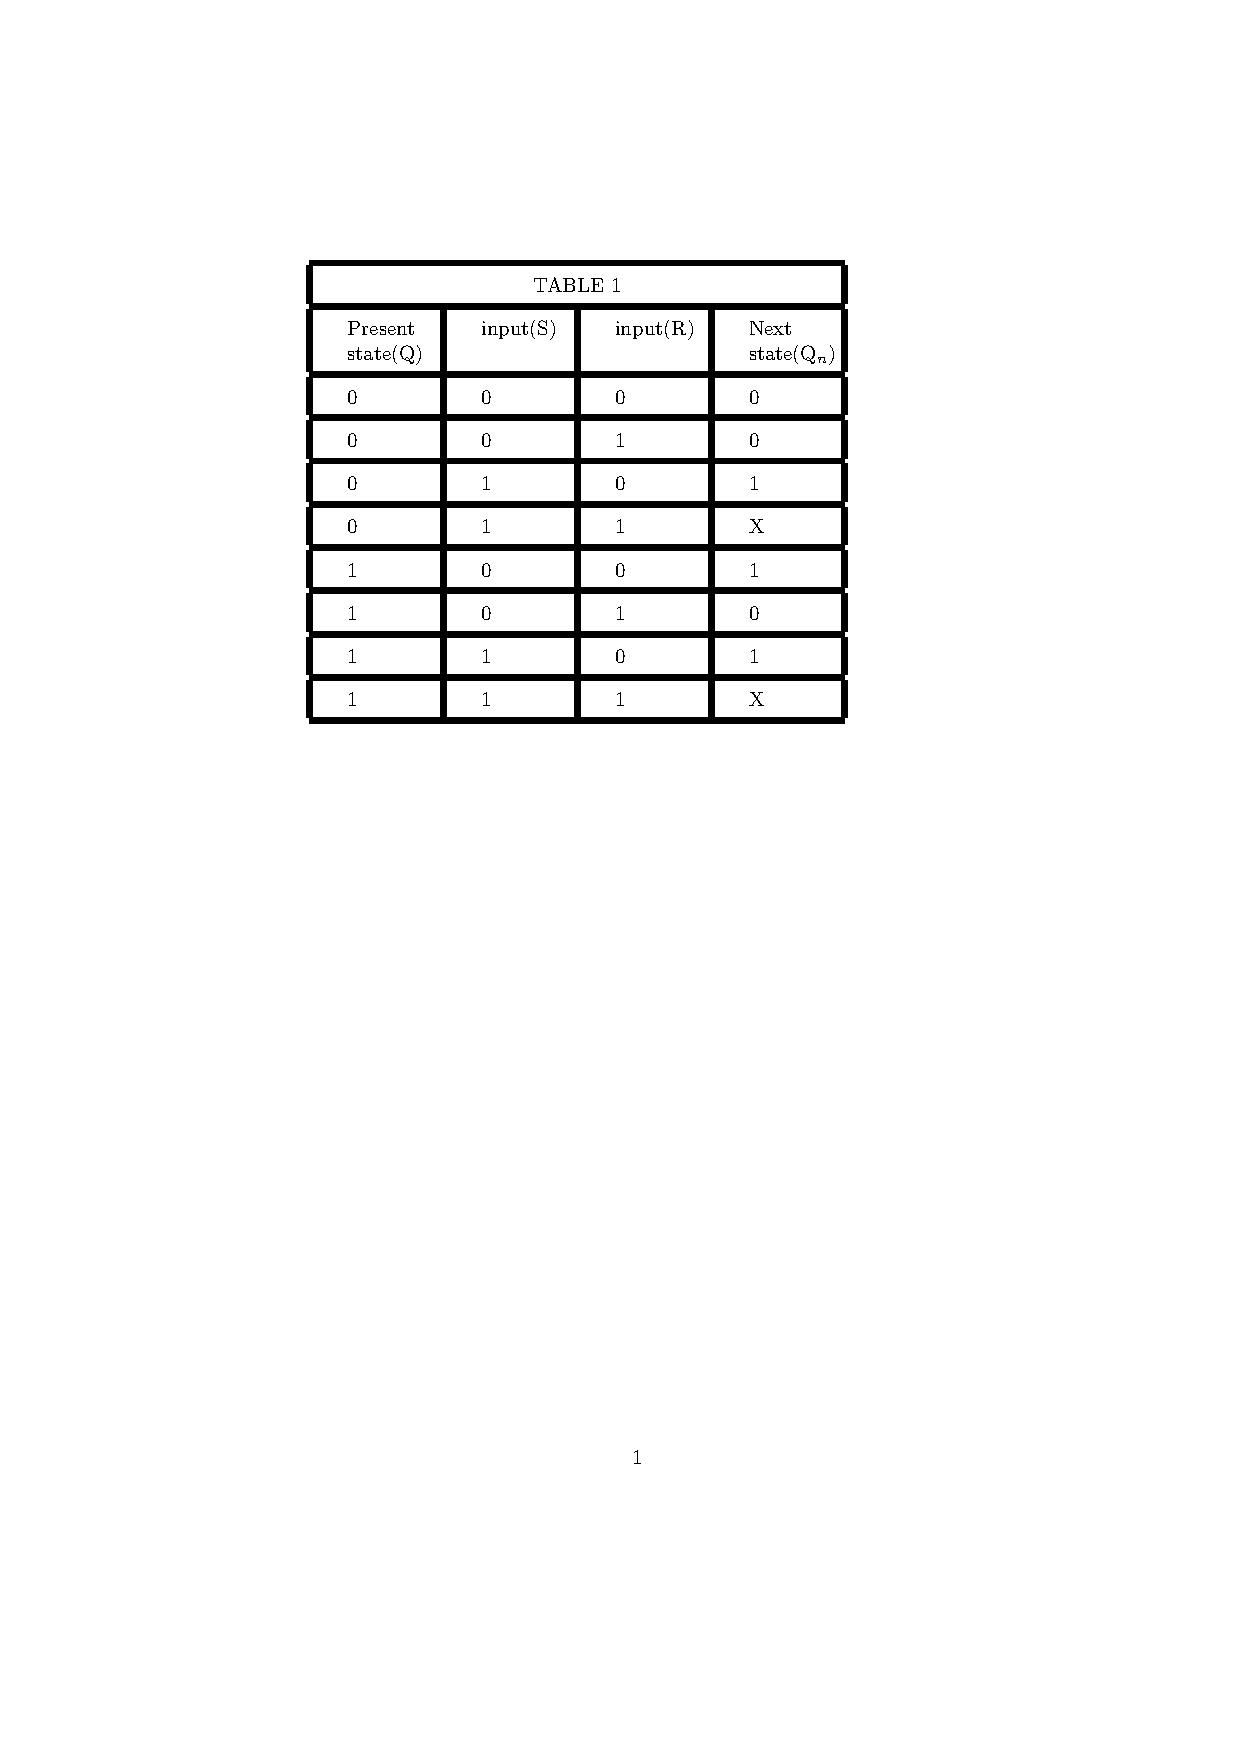
\includegraphics[width=400,height=400]{STATE_TRANSITION_TABLE.pdf}
\end{center}


\end{frame}
\subsection{TIMING DIAGRAM}
\begin{frame}
\frametitle{TIMING DIAGRAM}

\begin{center}
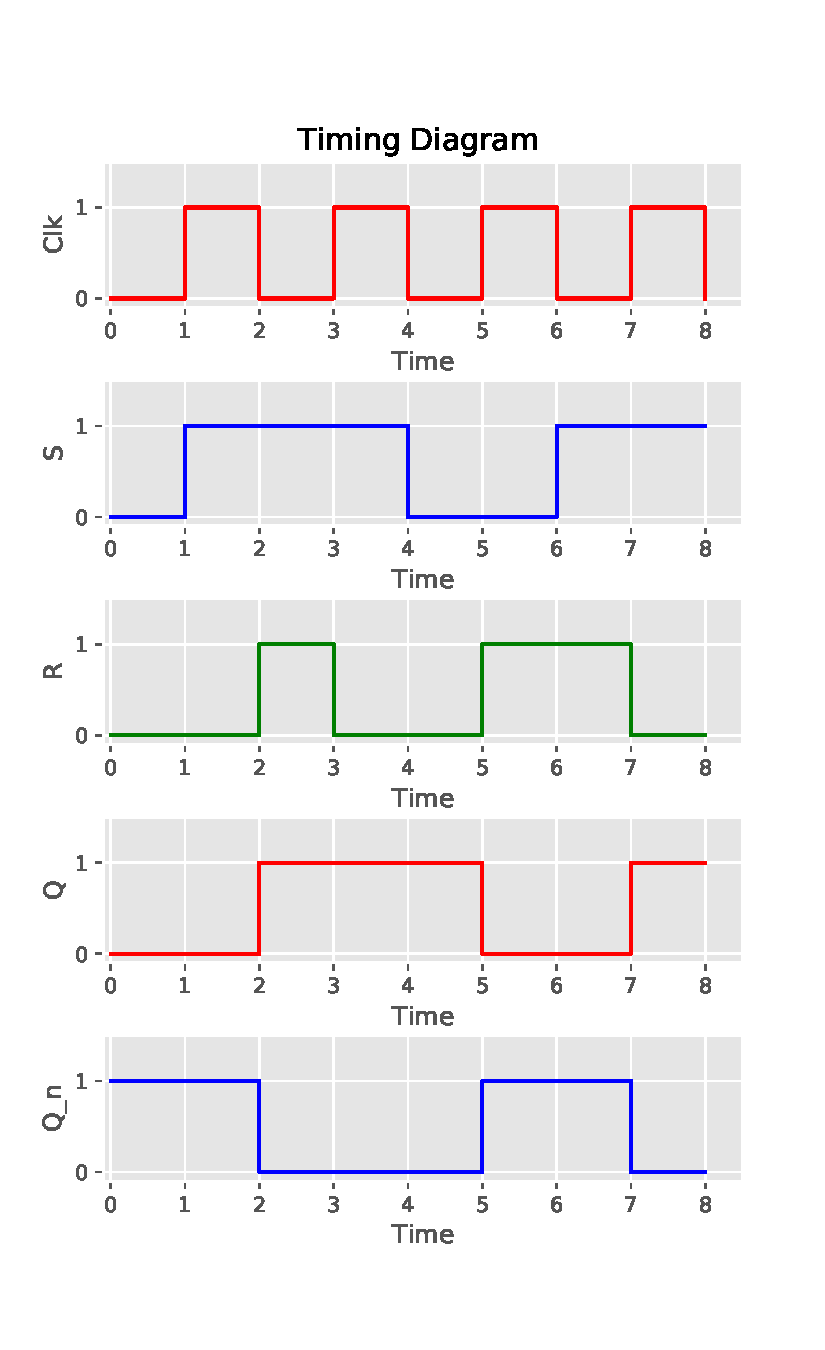
\includegraphics[width=200,height=200]{graph.pdf}
\end{center}


\end{frame}


\begin{frame}
\begin{center}
       \boldsymbol{THANKYOU}
\end{center}
\begin{center}
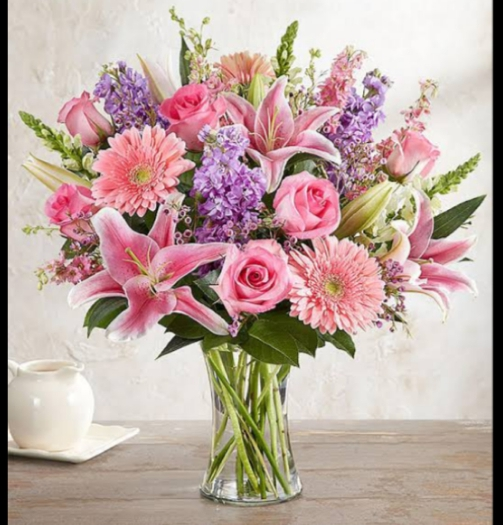
\includegraphics[width=100,height=100]{FLOWERS.jpeg}
\end{center}
\begin{corner}
\includegraphics[width=50,height=50]{gate.jpeg}
\end{corner}
\end{frame}


\end{document}